\documentclass[12pt]{report}
\usepackage[pdftex]{graphicx}
%\usepackage[pdftrex/bookmarksnumbered=true]{hyperref}
\usepackage{hyperref}
\linespread{1.5}
\textwidth = 6in
\textheight = 9in
\usepackage[body={6.0in, 8.2in},left=1.25in,right=1.0in,top=1.0in, bottom=1.0in]{geometry}
\frenchspacing
\usepackage{fancyhdr}
\usepackage{color}
\usepackage{xcolor}
\usepackage{listings}

\usepackage{caption}
\DeclareCaptionFont{white}{\color{white}}
\DeclareCaptionFormat{listing}{\colorbox{gray}{\parbox{\textwidth}{#1#2#3}}}
\captionsetup[lstlisting]{format=listing,labelfont=white,textfont=white}


\begin{document}
\pagenumbering{roman}
%\input{Coverpage.tex}

%----------------title page
\begin{titlepage}
\begin{center}
{\bf \large Decision Tree Classifier with GA based feature selection}\\
\vspace{.15in}
{\bfseries Mini Project Report}\\
\vspace{.15in}
{\normalsize Submitted to} \\
\vspace{.1in}
{\bfseries DEPARTMENT OF COMPUTER SCIENCE AND ENGINEERING}\\
\vspace{.25in}
{\normalsize \emph{By}}\\
{\bfseries\normalsize Samir Sheriff }\\
{\bfseries\normalsize Satvik N }\\
\vspace{.25in}
{\normalsize \emph{In partial fulfilment of the requirements\\ for the award of the degree \\
\vspace{.15in}
} } 

\vspace{.15in}
{\large{BACHELOR OF ENGINEERING}}\\
\vspace{.15in}
{\normalsize{IN}}\\
\vspace{.15in}
{\bfseries\normalsize COMPUTER SCIENCE AND ENGINEERING}\\
\vspace{0.15in}

\begin{figure}[h!]
	\centering
		\includegraphics[scale=0.5]{RVCE.png}
		
\end{figure} 
\vspace{.25in}
{\bfseries\large R V College of Engineering}\\
{\normalsize (Autonomous Institute, Affiliated to VTU)}\\
{\bfseries\normalsize BANGALORE - 560059}\\ 
{\bfseries\large May 2012}
\end{center}
\end{titlepage}


%---------Declaration
\begin{titlepage}
%\chapter*{\centerline{DECLARATION}}
\begin{center}
\section*{DECLARATION}
\end{center}

\paragraph{}  We, Samir Sheriff and Satvik N bearing USN number 1RV09CS093 and 1RV09CS095 respectively, hereby declare that the dissertation entitled ``\textbf{Decision Tree Classifier with GA feature selection}'' completed and written by us, has not been previously formed the basis for the award of any degree or diploma or certificate of any other University.
\vspace{1in}

\begin{flushright} {Bangalore \hspace{4.4in} Samir Sheriff } 
 {USN:1RV09CS093}
 \end{flushright}

\begin{flushright} { Satvik N } \\
 {USN:1RV09CS095}
 \end{flushright}
\end{titlepage}

%---------Certificate
\begin{titlepage}
\newpage
\begin{center}
{\bfseries\large R V COLLEGE OF ENGINEERING}\\
{\normalsize (Autonomous Institute Affiliated to VTU)}\\
{\normalsize DEPARTMENT OF COMPUTER SCIENCE AND ENGINEERING}\\
\end{center}
	
\begin{figure}[h!]
	\centering
		\includegraphics[scale=0.5]{RVCE.png}
		%\includegraphics{msrit-logo.jpg}
	%\caption{}
	%\label{fig:logo2}
\end{figure}

\begin{center}
\bf{\underline{CERTIFICATE}}
\end{center}
\noindent This is to certify that the dissertation entitled, ``\textbf{Decision Tree Classifier with GA based feature selection}'',  which is being submitted herewith for the award of B.E is the result of the work completed by \textbf{Samir Sheriff and Satvik N}  under my supervision and guidance.
\vspace{.5in}

\begin{flushleft} Signature of Guide 	
\\ (Name of the Guide) \\
\vspace{.5in}
 Signature of Head of Department  \hspace{4cm} Signature of Principal \\
 (Dr. N K Srinath) \hspace{6.6cm} (Dr. B.S Sathyanarayana)\\
 
 \end{flushleft} 
\begin{flushleft}
\hspace{1in}Name of Examiner \hspace{1.25in} Signature of Examiner
\end{flushleft}
\begin{flushleft}
1: \\
\vspace{.5in} 
2: 
\end{flushleft}
\end{titlepage}


%---------Acknowledgement
  
%\linespread{1.5}
\setcounter{page}{1}
\begin{center}
\section*{ACKNOWLEDGEMENT}
\addcontentsline{toc}{section}{ACKNOWLEDGEMENT}
\end{center}
The euphoria and satisfaction of the completion of the project will be incomplete
without thanking the persons responsible for this venture.


We acknowledge RVCE (Autonomous under VTU) for providing an opportunity to
create a mini-project in the 5th semester. We express our gratitude towards \textbf{Prof. B.S. Satyanarayana}, principal, R.V.C.E for constant encouragement and facilitates extended in completion of this project. We would like to thank \textbf{Prof. N.K.Srinath}, HOD, CSE
Dept. for providing excellent lab facilites for the completion of the project. We would
personally like to thank our project guides \textbf{Ms. Shantha Rangaswamy and Dr. } and also the lab in charge, for providing timely assistance \& guidance at the time.



We are indebted to the co-operation given by the lab administrators and lab assistants,
who have played a major role in bringing out the mini-project in the present form.
Bangalore



\begin{flushright}
Samir Sheriff\\
6th semester, CSE\\
USN:1RV09CS093\\

Satvik N\\
6th semester, CSE\\
USN:1RV09CS095\\

\end{flushright}

\newpage

%--------------Abstract
%\fontfamily{roman}%\selectfont
\begin{center}
\section*{ABSTRACT}
\addcontentsline{toc}{section}{ABSTRACT}
\end{center} 
The Project ``\textbf{Decision Tree based Classifier}” is aimed at developing programs that transform a string of characters in some representation (such as ASCII) into a new string (of bits, for example) which contains the same information but whose length is as small as possible.  Compression is useful because it helps reduce the consumption of resources such as data space or transmission capacity. The design of data compression schemes involve trade-off s among various factors, including the degree of compression, the amount of distortion introduced (e.g., when using lossy data compression), and the computational resources required to compress and uncompress the data.
 

Many data processing applications require storage of large volumes of data, and the number of such applications is constantly increasing as the use of computers extends to new disciplines.  Compressing data to be stored or transmitted reduces storage and/or communication costs. When the amount of data to be transmitted is reduced, the effect is that of increasing the capacity of the communication channel. Similarly, compressing a file to half of its original size is equivalent to doubling the capacity of the storage medium. It may then become feasible to store the data at a higher, thus faster, level of the storage hierarchy and reduce the load on the input/output channels of the computer system.



%------Table Of Contents
\addcontentsline{toc}{section}{CONTENTS}
\tableofcontents
%\listoffigures
%\listoftables


\newpage

\pagenumbering{arabic}
\setcounter{page}{1}

\pagestyle{fancy}
\lhead{\scriptsize{Introduction}}
\chead{}
\rhead{\scriptsize{Data Compression Techniques}}
\lfoot{\scriptsize{Dept. of CSE, R V C E, Bangalore.}}
\rfoot{\small{\thepage}}
\cfoot{\scriptsize{Feb 2012 - May 2013}}
\renewcommand{\headrulewidth}{0.4pt}
\renewcommand{\footrulewidth}{0.4pt}

\chapter{INTRODUCTION}

Trees are everywhere. We love trees.

\section{SCOPE}

The data compression techniques find applications in almost all fields. To list a few,
\begin{itemize}


\item{\textbf{Audio data compression}} reduces the transmission bandwidth and storage requirements of audio data. Audio compression algorithms are implemented in software as audio codecs. Lossy audio compression algorithms provide higher compression at the cost of fidelity, are used in numerous audio applications. These algorithms almost all rely on psychoacoustics to eliminate less audible or meaningful sounds, thereby reducing the space required to store or transmit them.
Video

\item{\textbf{Video compression}} uses modern coding techniques to reduce redundancy in video data. Most video compression algorithms and codecs combine spatial image compression and temporal motion compensation. Video compression is a practical implementation of source coding in information theory. In practice most video codecs also use audio compression techniques in parallel to compress the separate, but combined data streams.
\item{\textbf{Grammar-Based Codes}}

They can extremely compress highly-repetitive text, for instance, biological data collection of same or related species, huge versioned document collection, internet archives, etc. The basic task of grammar-based codes is constructing a context-free grammar deriving a single string. Sequitur and Re-Pair are practical grammar compression algorithms which public codes are available.
\end{itemize}


\pagestyle{fancy}
\lhead{\scriptsize{Software Requirements Specification}}
\chead{}
\rhead{\scriptsize{Data Compression Techniques}}
\lfoot{\scriptsize{Dept. of CSE, R V C E, Bangalore.}}
\rfoot{\small{\thepage}}
\cfoot{\scriptsize{Feb 2012 - May 2013}}
\renewcommand{\headrulewidth}{0.4pt}
\renewcommand{\footrulewidth}{0.4pt}
\chapter{REQUIREMENT SPECIFICATION}
Software Requirement Specification (SRS) is an important part of software development process. We describe about the overall description of the Data Compression Project, the specific requirements of the Data Compression Project, the software requirements and hardware requirements and the functionality of the system.





\subsubsection{Software Requirements}
\begin{itemize}

\item{	Front End: Qt GUI Application.}
\item{	Back End: C++}
\item{	Operating System: Linux.}

\end{itemize}

\subsubsection{Hardware Requirements}
\begin{itemize}
\item{Processor: Intel Pentium 4 or higher version}
\item{RAM: 512MB or more}
\item{Hard disk: 5 GB or less}
\end{itemize}

%\input{IMP.tex}
\pagestyle{fancy}
\lhead{\scriptsize{Compression}}
\chead{}
\rhead{\scriptsize{Data Compression Techniques}}
\lfoot{\scriptsize{Dept. of CSE, R V C E, Bangalore.}}
\rfoot{\small{\thepage}}
\cfoot{\scriptsize{Feb 2012 - May 2013}}
\renewcommand{\headrulewidth}{0.4pt}
\renewcommand{\footrulewidth}{0.4pt}
\chapter{Compression}



\section{A Naive Approach}

\begin{figure}[h!]
	\centering
		%\includegraphics[scale=0.7]{Table1.png}
		%\includegraphics{msrit-logo.jpg}
	%\caption{}
	%\label{fig:logo2}
\end{figure}

\section{The Basic Idea}


\section{Building the Huffman Tree}

\begin{itemize}

\item Begin with a forest of trees. All trees are one node, with the weight of the tree equal to the weight of the character in the node. Characters that occur most frequently have the highest weights. Characters that occur least frequently have the smallest weights.
\item    Repeat this step until there is only one tree:
\item    Choose two trees with the smallest weights, call these trees T1 and T2. Create a new tree whose root has a weight equal to the sum of the weights T1 + T2 and whose left subtree is T1 and whose right subtree is T2.
\item    The single tree left after the previous step is an optimal encoding tree..

\end{itemize}

\section{An Example}

\subsection{An Example: "go go gophers"}


\subsection{Example Encoding Table}

The character encoding induced by the last tree is shown below where again, 0 is used for left edges and 1 for right edges.

\begin{figure}[h!]
	\centering
		%\includegraphics[scale=0.7]{huffTable1.png}
		%\includegraphics{msrit-logo.jpg}
	%\caption{}
	%\label{fig:logo2}
\end{figure}

\subsection{Encoded String}

The string "go go gophers" would be encoded as shown (with spaces used for easier reading, the spaces wouldn't appear in the real encoding).
\textbf{00 01 100 00 01 100 00 01 1110 1101 101 1111 1100}

Once again, 37 bits are used to encode "go go gophers". There are several trees that yield an optimal 37-bit encoding of "go go gophers". The tree that actually results from a programmed implementation of Huffman's algorithm will be the same each time the program is run for the same weights (assuming no randomness is used in creating the tree).



\pagestyle{fancy}
\lhead{\scriptsize{Decompression}}
\chead{}
\rhead{\scriptsize{Data Compression Techniques}}
\lfoot{\scriptsize{Dept. of CSE, R V C E, Bangalore.}}
\rfoot{\small{\thepage}}
\cfoot{\scriptsize{Feb 2012 - May 2013}}
\renewcommand{\headrulewidth}{0.4pt}
\renewcommand{\footrulewidth}{0.4pt}

\chapter{Decompression}

Generally speaking, the process of decompression is simply a matter of translating the stream of prefix codes to individual byte values, usually by traversing the Huffman tree node by node as each bit is read from the input stream (reaching a leaf node necessarily terminates the search for that particular byte value). Before this can take place, however, the Huffman tree must be somehow reconstructed.

\section{Storing the Huffman Tree}

\begin{itemize}
\item In the simplest case, where character frequencies are fairly predictable, the tree can be preconstructed (and even statistically adjusted on each compression cycle) and thus reused every time, at the expense of at least some measure of compression efficiency.

\item Otherwise, the information to reconstruct the tree must be sent a priori.

\item A naive approach might be to prepend the frequency count of each character to the compression stream. Unfortunately, the overhead in such a case could amount to several kilobytes, so this method has little practical use.

\item Another method is to simply prepend the Huffman tree, bit by bit, to the output stream. For example, assuming that the value of 0 represents a parent node and 1 a leaf node, whenever the latter is encountered the tree building routine simply reads the next 8 bits to determine the character value of that particular leaf. The process continues recursively until the last leaf node is reached; at that point, the Huffman tree will thus be faithfully reconstructed. The overhead using such a method ranges from roughly 2 to 320 bytes (assuming an 8-bit alphabet). 

\begin{figure}[h!]
	\centering
		%\includegraphics[scale=0.7]{hufftreedecomp.png}
		%\includegraphics{msrit-logo.jpg}
	%\caption{}
	%\label{fig:logo2}
\end{figure}

\end{itemize}

Many other techniques are possible as well. In any case, since the compressed data can include unused "trailing bits" the decompressor must be able to determine when to stop producing output. This can be accomplished by either transmitting the length of the decompressed data along with the compression model or by defining a special code symbol to signify the end of input (the latter method can adversely affect code length optimality, however).


\section{Creating the Huffman Table}

To create a table or map of coded bit values for each character you'll need to traverse the Huffman tree (e.g., inorder, preorder, etc.) making an entry in the table each time you reach a leaf. For example, if you reach a leaf that stores the character 'C', following a path left-left-right-right-left, then an entry in the 'C'-th location of the map should be set to 00110. You'll need to make a decision about how to store the bit patterns in the map. At least two methods are possible for implementing what could be a class/struct BitPattern: 

\begin{itemize}

\item    Use a string. This makes it easy to add a character (using +) to a string during tree traversal and makes it possible to use string as BitPattern. Your program may be slow because appending characters to a string (in creating the bit pattern) and accessing characters in a string (in writing 0's or 1's when compressing) is slower than the next approach.

\item    Alternatively you can store an integer for the bitwise coding of a character. You need to store the length of the code too to differentiate between 01001 and 00101. However, using an int restricts root-to-leaf paths to be at most 32 edges long since an int holds 32 bits. In a pathological file, a Huffman tree could have a root-to-leaf path of over 100. Because of this problem, you should use strings to store paths rather than ints. A slow correct program is better than a fast incorrect program. 

\end{itemize}

\section{Storing Sizes}

The operating system will buffer output, i.e., output to disk actually occurs when some internal buffer is full. In particular, it is not possible to write just one single bit to a file, all output is actually done in "chunks", e.g., it might be done in eight-bit chunks. In any case, when you write 3 bits, then 2 bits, then 10 bits, all the bits are eventually written, but you can not be sure precisely when they're written during the execution of your program. Also, because of buffering, if all output is done in eight-bit chunks and your program writes exactly 61 bits explicitly, then 3 extra bits will be written so that the number of bits written is a multiple of eight. Because of the potential for the existence of these "extra" bits when reading one bit at a time, you cannot simply read bits until there are no more left since your program might then read the extra bits written due to buffering. This means that when reading a compressed file, you CANNOT use code like this.

\begin{verbatim}
	int bits; 
	while (input.readbits(1, bits)) 
	{ 
		// process bits 
	} 
\end{verbatim}



To avoid this problem, you can write the size of a data structure before writing the data structure to the file.
\pagestyle{fancy}
\lhead{\scriptsize{Conclusion}}
\chead{}
\rhead{\scriptsize{Data Compression Techniques}}
\lfoot{\scriptsize{Dept. of CSE, R V C E, Bangalore.}}
\rfoot{\small{\thepage}}
\cfoot{\scriptsize{Feb 2012 - May 2013}}
\renewcommand{\headrulewidth}{0.4pt}
\renewcommand{\footrulewidth}{0.4pt}
\chapter{CONCLUSION AND FUTURE WORKS}

\textbf{Summary}

\textbf{Limitations}
\begin{enumerate}
\item{Huffman code is optimal only if exact probability distribution of the source symbols is known.}
 
\item{Each symbol is encoded with integer number of bits.}
 
\item{Huffman coding is not efficient to adapt with the changing source statistics.}
 \item{The length of the codes of the least probable symbol could be very large to store into a single word or basic storage unit in a computing system.}
\end{enumerate}
	\textbf{Further enhancements}
The huffman coding the we have considered is simple binary Huffman codingbut many variations of Huffman coding exist,
\begin{enumerate}

\item{\textbf{ n-ary Huffman coding: }} The n-ary Huffman algorithm uses the \{0, 1, ... , n − 1\} alphabet to encode message and build an n-ary tree. This approach was considered by Huffman in his original paper. The same algorithm applies as for binary (n equals 2)codes, except that the n least probable symbols are taken together, instead of just the 2 least probable. Note that for n greater than 2, not all sets of source words can properly form an n-ary tree for Huffman coding. In this case, additional 0-probability place holders must be added. If the number of source words is congruent to 1 modulo n-1, then the set of source words will form a proper Huffman tree.
\item{\textbf{Adaptive Huffman coding: }}A variation called adaptive Huffman coding calculates the probabilities dynamically based on recent actual frequencies in the source string. This is some what related to the LZ family of algorithms.
\item{\textbf{Huffman template algorithm: }}Most often, the weights used in implementations of Huffman coding represent numeric probabilities, but the algorithm given above does not require this; it requires only a way to order weights and to add them. The Huffman template algorithm enables one to use any kind of weights (costs,frequencies etc)
\item{\textbf{Length-limited Huffman coding: }}Length-limited Huffman coding is a variant where the goal is still to achieve a minimum weighted path length, but there is an additional restriction that the length of each codeword must be less than a given constant. The package-merge algorithm solves this problem with a simple greedy approach very similar to that used by Huffman's algorithm. Its time complexity is O(nL),where L is the maximum length of a codeword. No algorithm is known to solve this problem in linear or linear logarithmic time, unlike the presorted and unsorted conventional Huffman problems, respectively.
%\item{\textbf{Huffman coding with unequal letter costs: }}Huffman coding with unequal letter costs is the generalization in which this assumption is no longer assumed true: the letters of the encoding alphabet may have non-uniform lengths, due to characteristics of the transmission medium. An example is the encoding alphabet of Morse code, where a 'dash' takes longer to send than a 'dot', and therefore the cost of a dash in transmission time is higher. The goal is still to minimize the weighted average codeword length,but it is no longer sufficient just to minimize the number of symbols used by the message. No algorithm is known to solve this in the same manner or with the same efficiency as conventional Huffman coding.Moreover we can extend the range of the huffman coding software to in corporate unicode which will require an interfacing module that will interpret a particular key in different languages based on the option selected. In that case the maximum number of symbols will be of the order of $2^{32}$
\end{enumerate}

\newpage

%For Bib refer to refs.bib to add/remove bib items
\addcontentsline{toc}{section}{BIBLIOGRAPHY}
\begin{thebibliography}{refs}
\bibitem{test}Genetic Algorithms  -\url{http://en.wikipedia.org/wiki/Genetic_algorithm}
\bibitem{t}Genetic Algorithm for constructing DT - \url{http://www.jprr.org/index.php/jprr/article/viewFile/44/25}
%\bibtitem{te}Decision Trees - \url{http://web.cecs.pdx.edu/~mm/MachineLearningWinter2010/pdfslides/DecisionTrees.pdf}
\bibitem{t} Project brief for the DT  using Horse data sets  - \url{https://cs.uwaterloo.ca/~ppoupart/teaching/cs486-spring06/assignments/asst4/asst4.pdf}
\bibitem{t}Supervised and Unsupervised Discretization of Continous Features - \url{http://robotics.stanford.edu/users/sahami/papers-dir/disc.pdf}
\bibitem{t}Hybrid learning using Genetic Algorithms and Decision Trees for pattern sification - \url{http://cs.gmu.edu/~eclab/papers/ijcai95.pdf}
\bibitem{t}Kardi Maams' Tutorials - \url{http://people.revoledu.com/kardi/tutorial/DecisionTree/index.html}

%\bibitem{}
%\bibitem{}
\end{thebibliography}

\newpage
\pagestyle{fancy}
\lhead{\scriptsize{Appendix A: Source Code}}
\chead{}
\rhead{\scriptsize{Data Compression Techniques}}
\lfoot{\scriptsize{Dept. of CSE, R V C E, Bangalore.}}
\rfoot{\small{\thepage}}
\cfoot{\scriptsize{Feb 2012 - May 2013}}
\renewcommand{\headrulewidth}{0.4pt}
\renewcommand{\footrulewidth}{0.4pt}

\addcontentsline{toc}{section*}{APPENDICES}
\section*{Appendices}
\section*{Appendix A : Source Code}
%\begin{lstinputlisting}[label=some-code,caption=Some Code]{Charnode.h}
%\lstinputlisting[ language=C++, label=charnode, caption=The definiton of the class Charnode\, each node of the huffman tree is an object of this class.]{Charnode.h}
%
%\lstinputlisting[language=C++, label=huffman,caption=The definition  of the class Huffman\, this class helps in building the huffman tree for an input file.]{HuffmanCode.h}
%
%\lstinputlisting[language=C++, label=compresswrite,caption=The definition  of the class CompressionWriting\, this class helps in writing the bits to the compressed file.]{CompressionWriting.h}
%
%\lstinputlisting[language=C++, label=huff,caption=The main program of the huffman compression algorithm.]{huff.cpp}
%
%\lstinputlisting[language=C++, label=unhuff,caption=The definition of the class Decompressor\, this class helps in decompressing the compressed file using huffman algorithm.]{Decompressor.h}
%
%\lstinputlisting[language=C++, label=unhuff,caption=The main program of the huffman decompression algorithm.]{unhuff.cpp}


%\lstinputlisting[language=C++, label=unhuff,caption=The definition of the class TCP\_Server\, an object of this class is a server object that can concurrently handle requests for files from the clients.]{TCP_Server.h}

%\lstinputlisting[language=C++, label=unhuff,caption=The definition of the class TCP\_Client\, an object of this class indicates a client object that can request for files from the server.]{TCP_Client.h}


\newpage
\pagestyle{fancy}
\lhead{\scriptsize{Appendix B: Screen shots}}
\chead{}
\rhead{\scriptsize{Decision Tree Classifier}}
\lfoot{\scriptsize{Dept. of CSE, R V C E, Bangalore.}}
\rfoot{\small{\thepage}}
\cfoot{\scriptsize{Sep 2012 - May 2013}}
\renewcommand{\headrulewidth}{0.4pt}
\renewcommand{\footrulewidth}{0.4pt}


\section*{Appendix B : Screen Shots}
\begin{figure}[h!]

  \centering
    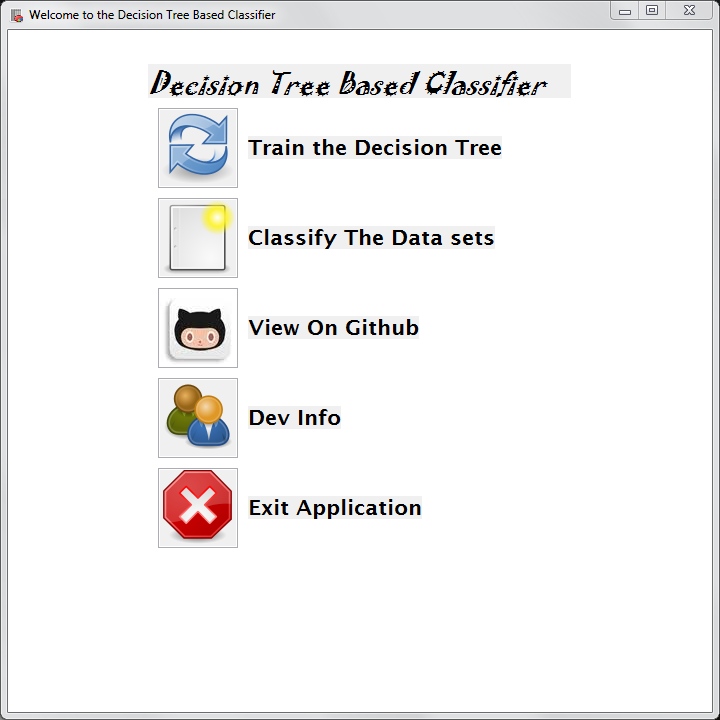
\includegraphics[scale=0.40]{welcome_window.png}
  \caption{Application Window - Welcome Screen}
\end{figure}

\begin{figure}[h!]
  
  \centering
    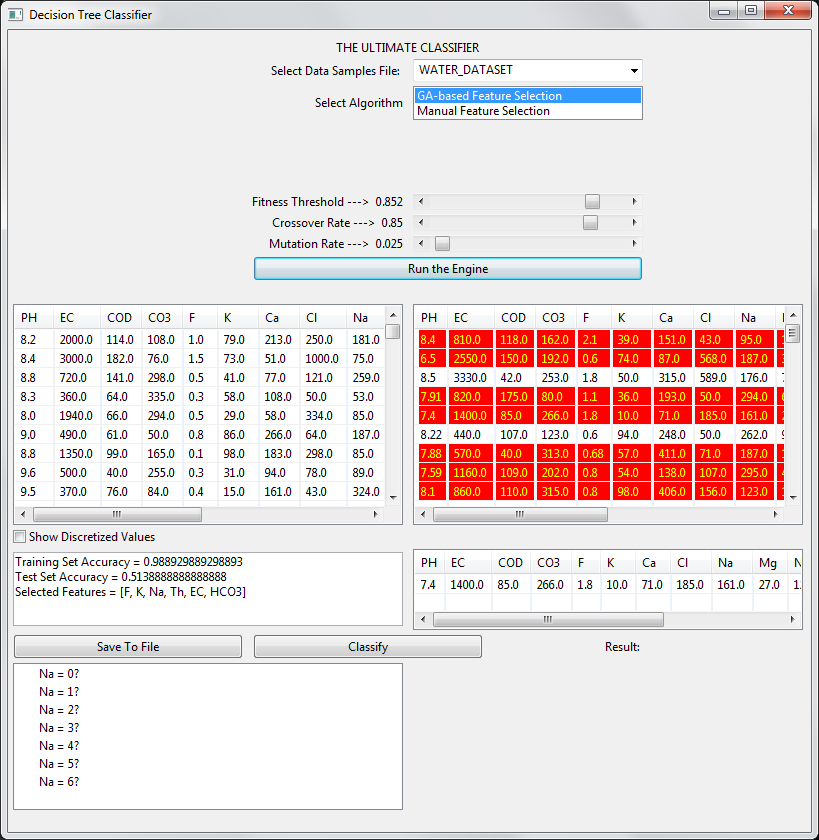
\includegraphics[scale=0.45]{dt_classifier.png}
\caption{Decision Tree Constructor Window.}
\end{figure}

\begin{figure}[h!]
  
  \centering
    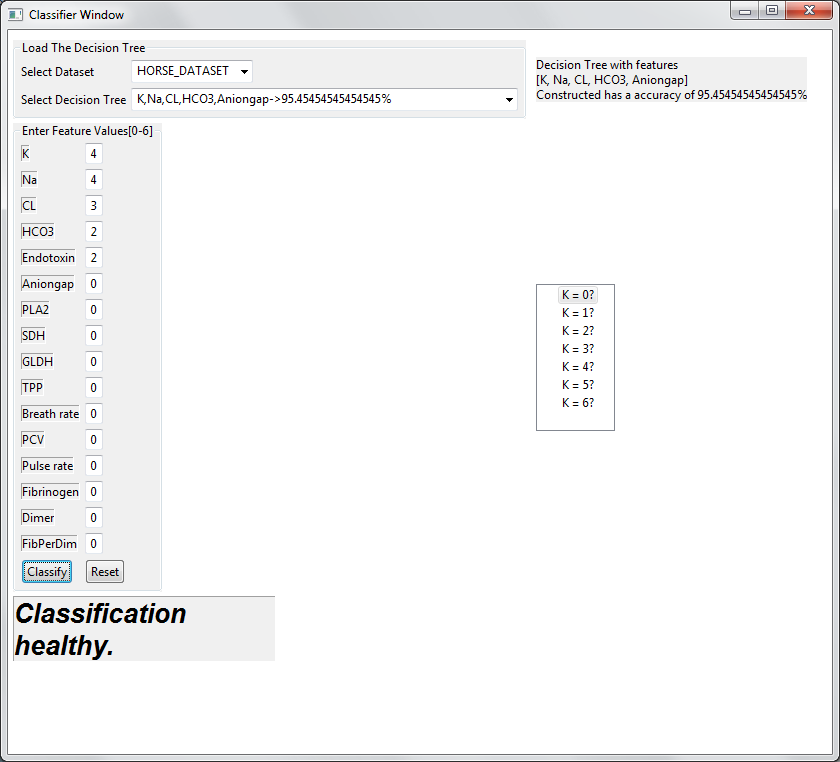
\includegraphics[scale=0.45]{dt_classification_window.png}
\caption{Decision Tree Classifier Window.}
\end{figure}
\begin{figure}[h!]
  
  \centering
    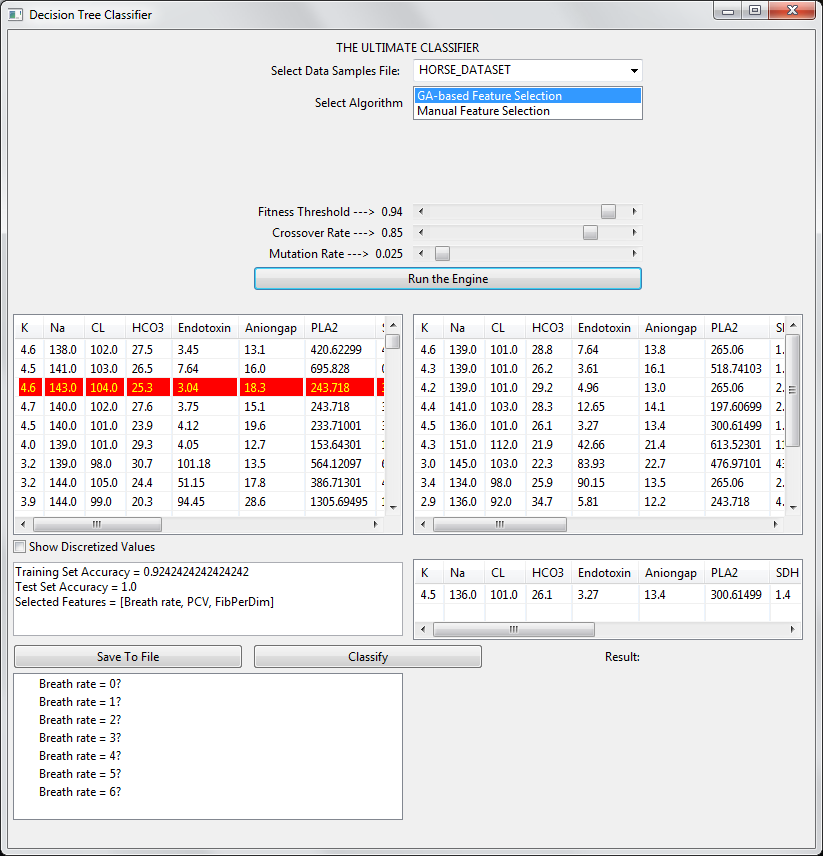
\includegraphics[scale=0.45]{dt_ga_algorithm.png}
\caption{Decision Tree Construction with GA based Feature Selector.}
\end{figure}

\begin{figure}[h!]
  
  \centering
    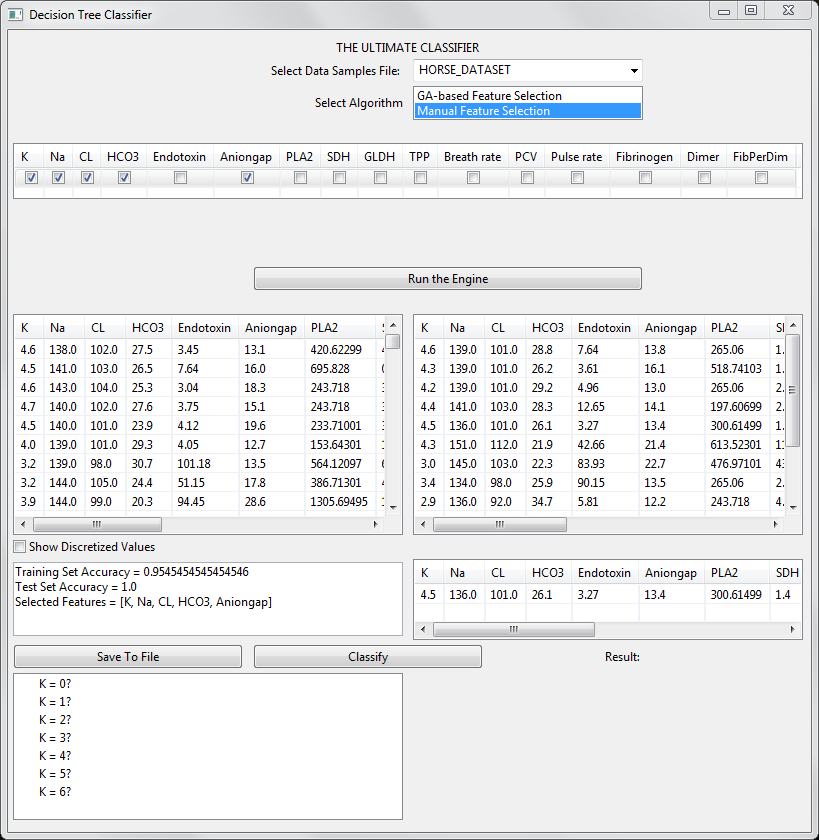
\includegraphics[scale=0.45]{dt_manual_selection.png}
\caption{Decision Tree Construction with manual feature selection.}
\end{figure}

\begin{figure}[h!]
  
  \centering
    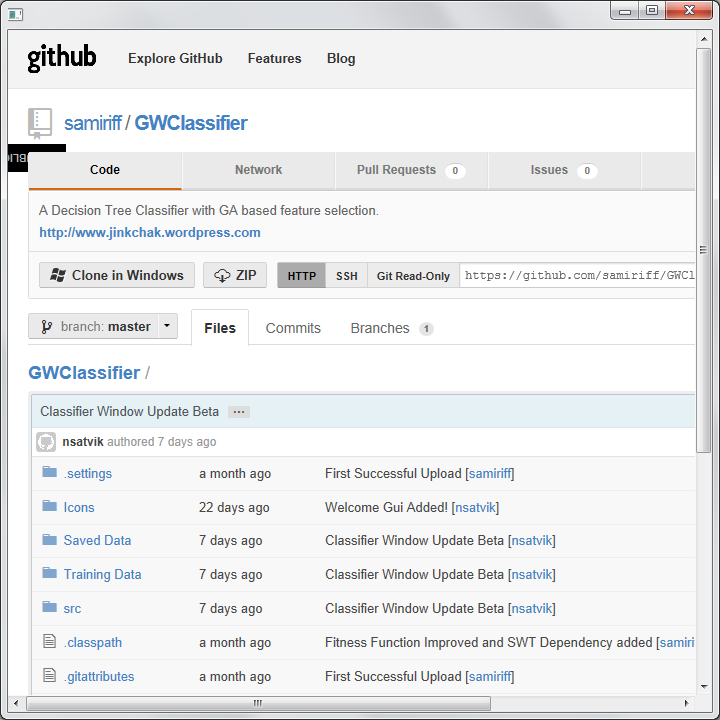
\includegraphics[scale=0.45]{git_hub.png}
\caption{The project source code on github public repository.}
\end{figure}


\end{document}
